\chapter{Systemarchitektur und Implementierung}

  Dieses Kapitel beschreibt die technische Umsetzung des entwickelten KI-gestützten Assistenzsystems zur quantitativen Portfoliooptimierung.
  Im Mittelpunkt stehen dabei der Aufbau der Softwarearchitektur, die verwendeten Technologien sowie die konkreten Implementierungsschritte.

  Ziel ist es, die Struktur und das Zusammenspiel der einzelnen Systemkomponenten nachvollziehbar darzustellen und zentrale Entwurfsentscheidungen zu begründen.
  Neben einer modularen Systemdarstellung werden auch technische Herausforderungen, etwa hinsichtlich Antwortlatenzen oder Schnittstellendefinitionen, aufgezeigt.
  Weiterhin werden die verwendeten Frameworks und Tools dokumentiert, um eine vollständige technische Nachvollziehbarkeit sicherzustellen.

  \section{Überblick über die Systemarchitektur}

    Das entwickelte Assistenzsystem zur quantitativen Portfoliooptimierung basiert auf einer modularen Client-Server-Architektur.
    Der gesamte Software-Stack gliedert sich in mehrere logische Komponenten, die sowohl funktional als auch technologisch getrennt implementiert wurden.
    Die Architektur gewährleistet eine klare Trennung von Zuständigkeiten sowie eine einfache Erweiterbarkeit einzelner Module (siehe Abbildung~\ref{fig:systemarchitektur}).

    \begin{figure}[h]
        \centering
        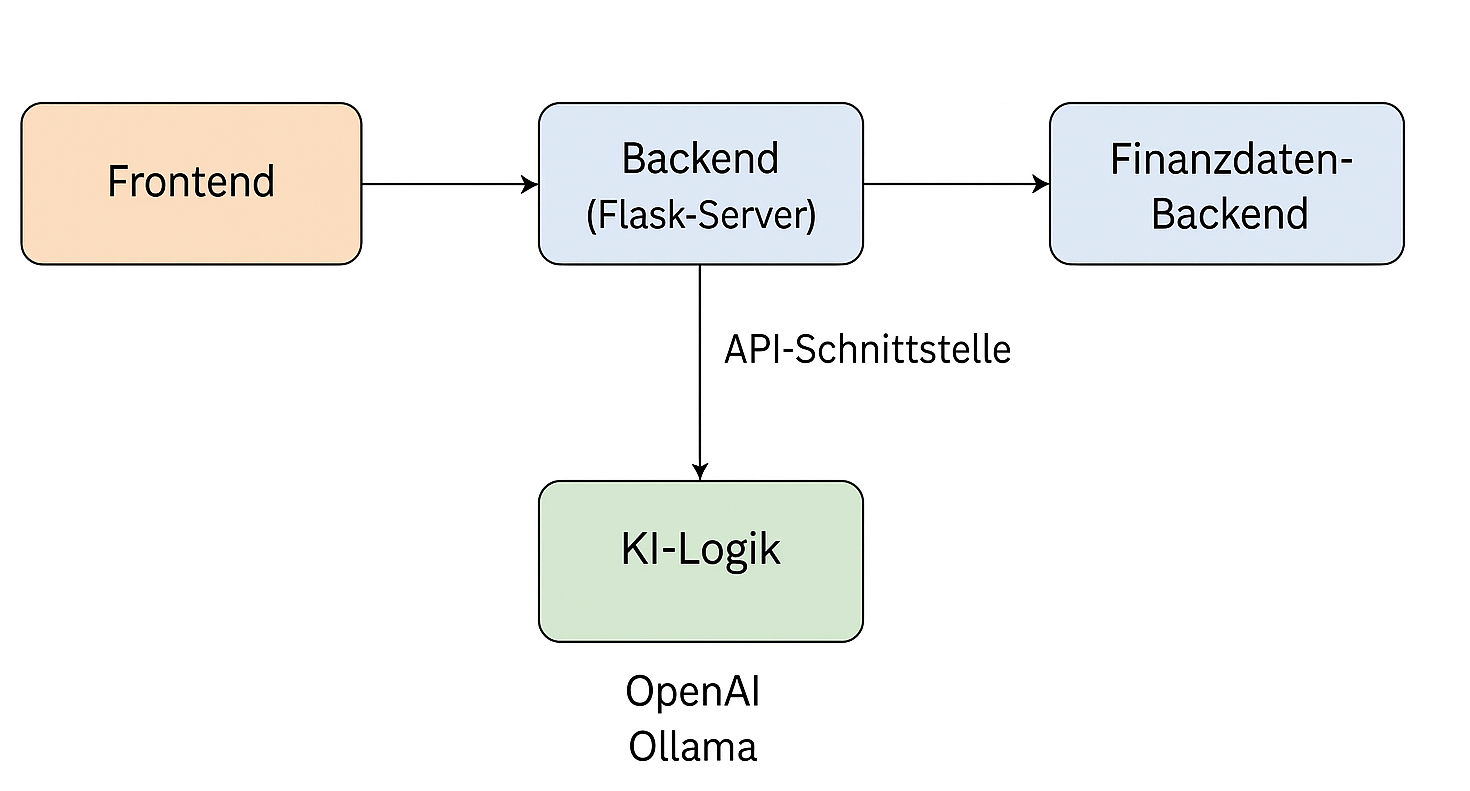
\includegraphics[width=\textwidth]{assets/pictures/vereinfachte_systemarchitektur.png}
        \caption{Modulare Systemarchitektur des KI-Assistenzsystems in vereinfachter Form}
        \label{fig:systemarchitektur}
    \end{figure}

    \subsection{Komponentenübersicht und Schnittstellen}

      Die Systemarchitektur besteht aus den folgenden Hauptkomponenten:

      \begin{itemize}
          \item \textbf{Backend (Flask-Server):} Das Backend ist in \texttt{Python} realisiert und stellt RESTful-Endpunkte für das Frontend bereit.
          Es orchestriert die Kommunikation mit dem LLM (Large Language Model), führt die Datenanalyse durch und verwaltet Persistenzstrukturen in JSON-Format.
          Hierzu wurde das \texttt{Flask}-Framework verwendet.

          \item \textbf{KI-Logik (LLM-Modul):} Die Analyse der Portfolios erfolgt durch Integration von LLMs, initial lokal mit \texttt{Ollama} um den On-Device-Ansatz zu verfolgen, später ergänzt durch eine API-Schnittstelle zur Anbindung von größeren und schnelleren Modellen von OpenAI.
          Die Auswahl des LLM-Anbieters ist modular über das \texttt{llm.py}-Modul steuerbar.
          Die Entscheidungsbegründungen werden extrahiert, strukturiert und transparent in das Portfolio eingebettet.

          \item \textbf{Finanzdaten-Backend:} Für die zeitnahe Beschaffung historischer und aktueller Finanzdaten wird das Python-Modul \texttt{yfinance} eingesetzt.
          Es dient als zentrale Datenquelle für Kursinformationen.

          \item \textbf{Frontend:} Das Frontend basiert auf einfachem \texttt{HTML} mit \texttt{Bootstrap} und \texttt{JavaScript}, welches über Flask bereitgestellt wird und mit dynamischen Elementen zur die Visualisierung und Präsentation der Handlungsempfehlungen zugängerlicher macht.
          Die UI verwendet asynchrone API-Aufrufe zur Aktualisierung der dargestellten Inhalte in Echtzeit.

          \item \textbf{LangChain:} Neben den direkten Aufrufen der LLM über die API Richtung Ollama oder Online-Anbietern ist die Integration von \texttt{LangChain} zur feineren Modellsteuerung und Verkettung von LLM-Aufrufen implementiert. Etwa für multi-step Reasoning über Zeit.
      \end{itemize}

      Alle Komponenten kommunizieren über klar definierte Schnittstellen.
      Dazu werden JSON-basierte Datenstrukturen über HTTP-Endpunkte genutzt.
      Dies ermöglicht die spätere Substitution einzelner Module (z. B. andere Frontends oder LLM-Anbieter).

  \section{Entwicklungsverlauf und iterative Verbesserung}

    Die Entwicklung des Systems erfolgte in iterativen Schritten, beginnend mit einem simplen Konsolen-Backend, welches sukzessive erweitert wurde.
    Der Fortschritt lässt sich grob in folgende Meilensteine unterteilen:

    \begin{enumerate}
        \item \textbf{Initiale Projektstrukturierung:} In der ersten Phase wurde ein minimales Backend eingerichtet, bestehend aus den Dateien \texttt{server.py}, \texttt{llm.py} und \texttt{main.py} (\textit{Commit: 3d6d728e51d4cef01ebf949b339af8a066a257f1}).
        Ziel war es, eine funktionale Basis für spätere Erweiterungen zu schaffen.

        \item \textbf{Entkopplung und Modularisierung des LLM-Moduls:} Die Datei \texttt{llm.py} wurde zunächst stark vereinfacht, um den Fokus auf den Aufbau eines separaten Moduls zur Portfoliobewertung in \texttt{portfolio\_ai.py} zu legen (\textit{Commit: ba1e79dc545d4020ab6fbddbbc50528a52225824}).
        Erste Dummy-Funktionen wurden eingeführt.

        \item \textbf{Extraktion von Modellantworten und JSON-Verarbeitung:} Das System wurde um die Fähigkeit erweitert, strukturierte JSON-Antworten aus den generierten Texten der LLMs zu extrahieren und weiterzuverarbeiten (\textit{Commit: 0c6299b410299bd581bdf9514a59e734790e7c78}).

        \item \textbf{Einbindung qualitativer Bewertungsdaten:} Erste Analysemethoden für Aktienportfolios wurden implementiert.
        Qualitative Merkmale wurden in die Bewertung einbezogen (\textit{Commit: 936e1a482756c678843262be903d3df8d5b0c06c}).

        \item \textbf{Erste Visualisierungsideen im HTML-Frontend:} Ein erster Entwurf des UI wurde eingebettet in die \texttt{server.py}-Datei umgesetzt. Die Ergebnisse der KI-Auswertung wurden rudimentär im Browser dargestellt (\textit{Commit: c5431d4e539bfa59349464e7fab9fddf0bb10fd3}).

        \item \textbf{Trennung von Frontend-Komponenten:} HTML, CSS und JavaScript wurden in separate Dateien ausgelagert, wodurch die Wartbarkeit verbessert und der Weg für komplexere UI-Funktionalität geebnet wurde (\textit{Commit: fa7e330adcc6a7ad3024d4465e94a55e5bd17f8a}).

        \item \textbf{Erweiterung der Benutzeroberfläche:} Es wurden Tabs für einzelne Aktienpositionen, modale Dialoge zur Konfiguration und Refresh-Buttons zur Aktualisierung des Portfolios implementiert (\textit{Commit: 1e3e01b2c22cd937d19ce55e32aee2f17de9dfbf}, \textit{7d7efd8d3dcfd9fba1b3c0d41c7a308fbe397479}).

        \item \textbf{Integration der API-Kommunikation:} Eine asynchrone Kommunikation zwischen Frontend und Backend wurde realisiert.
         Die JavaScript-Klasse in \texttt{api.js} übernahm dabei die zentrale Steuerung der Interaktion mit der Python-API (\textit{Commit: 0b68f880eacbdaa2cf4632a342aa8b5f206b4b76}).

        \item \textbf{Verbesserung der Portfoliostruktur:} Eine strukturierte JSON-Repräsentation des Portfolios wurde entworfen und eingeführt, um konsistente Datenhaltung für Bewertungen und Visualisierungen sicherzustellen (\textit{Commit: 347734ed2d1f22f025b44cd2488a721c942d78c0}).

        \item \textbf{Erweiterte Testdaten und dynamisches UI-Binding:} Die Oberfläche wurde mit dynamischen DOM-Manipulationen angereichert, z.\,B. zur Anzeige von Aktieninformationen, Dringlichkeitskennzahlen und historischen Vergleichsdaten.
        Dazu wurden auch exemplarische Testdaten angepasst (\textit{Commits: 7ee3eb6c1b765e3894c49664f5f8a811930ad9c7}, \textit{5e37f00105c9ec69edc2822423829f8235f34193}).

        \item \textbf{Persistenz und Rückschreibelogik:} Die Portfoliobewertungen wurden gespeichert, um wiederholte Analysen zu ermöglichen.
        Persistenz wurde durch Aktualisierung der JSON-Daten sichergestellt (\textit{Commit: 5e37f00105c9ec69edc2822423829f8235f34193}).

        \item \textbf{Fehlerbehandlung und Logging:} Zur besseren Nachvollziehbarkeit wurden umfassende Logging-Funktionen implementiert.
        Fehler beim Parsen von Antworten und bei Latenzen wurden protokolliert (\textit{Commit: 804fc3024699cac968c26f286f9c78fbb06014dc}).

        \item \textbf{Mehrfachmodell-Unterstützung für LLMs:} Neben Ollama wurde ein schnellerer Online-LLM integriert, um Antwortzeiten zu optimieren und die Auswahl geeigneter Modelle zu erleichtern (\textit{Commit: 734bf0010b3bf6cb9cceac52373d726fa23d6534}).

        \item \textbf{Finale UI-Optimierungen:} Die Interaktion wurde verfeinert durch Refresh-Buttons, Identifier für einzelne Elemente und erweiterte Tab-Logik.
        Frontend und Backend sind nun durch eine stabile API vollständig entkoppelt (\textit{Commit: 211026820610ea62ab2e4eeb7d9ab3a2188ab6d5}).
    \end{enumerate}

  \section{Technische Limitationen und Herausforderungen}

    Trotz modularer Architektur und performanter Tools bestehen derzeit folgende technische Limitationen:

    \begin{itemize}
        \item \textbf{Latenzzeiten bei LLM-Antworten:} Der Einsatz lokaler Modelle (Ollama) kann zu spürbaren Antwortverzögerungen führen, da die lokale Hardware weniger performant ist. Online Modelle wie von OpenAI bieten hier eine schnellere Alternative, bringen jedoch andere Einschränkungen hinsichtlich Datenschutz und Kosten mit sich.

        \item \textbf{Skalierung der Frontend-Interaktivität:} Mit wachsender Datenmenge steigt die Komplexität in der UI-Verwaltung.

        \item \textbf{Fehlende Parallelisierung:} Aktuell sind LLM-Anfragen sequentiell implementiert. Zur Beschleunigung könnten multiprocessing- oder queue-basierte Architekturen genutzt werden.

        \item \textbf{Erklärbarkeit:} Die Generierung der Begründungen basiert auf der natürlichen Sprache des LLMs, was trotz Parsingmaßnahmen keine formale Verifikation erlaubt.
    \end{itemize}

  \section{Eingesetzte Frameworks und Technologien}

    Die Implementierung stützt sich auf eine Vielzahl etablierter Open-Source-Frameworks:

    \begin{itemize}
        \item \texttt{Flask} – Python-Webframework für REST-APIs
        \item \texttt{Ollama} – Lokale Ausführung von LLMs für niedrigere Latenz
        \item \texttt{OpenAI API} – Anbindung an GPT-Modelle zur Entscheidungsfindung
        \item \texttt{yfinance} – Datenbeschaffung von historischen und aktuellen Kursdaten
        \item \texttt{LangChain} – Zur Verarbeitung komplexer Modellabläufe
        \item \texttt{Bootstrap} – Design-Framework zur responsiven UI-Gestaltung
        \item \texttt{JavaScript} – Logik und DOM-Manipulation im Browser
    \end{itemize}

  \section{Dokumentation und Erläuterung der Programmlogik}

    Nachfolgend werden exemplarische Platzhalter für Code-Auszüge angegeben, die im weiteren Verlauf der Arbeit durch echte Implementierungen ersetzt werden:

    \begin{lstlisting}[language=Python, caption=API-Endpunkt zur Portfoliobewertung]
      // Platzhalter
    \end{lstlisting}

    \begin{lstlisting}[caption=Asynchrone API-Kommunikation im Frontend]
      // Platzhalter
    \end{lstlisting}

  \section{Frontend}

    \subsection{Konzeptioneller Entwurf}

      Die Gestaltung des Frontends spielt eine zentrale Rolle in der Entwicklung von Assistenzsystemen, insbesondere dann, wenn es darum geht, komplexe algorithmische Empfehlungen für menschliche Nutzer nachvollziehbar und vertrauenswürdig zu präsentieren.
      Bereits zu Beginn der Entwicklung wurde ein grafischer Entwurf erstellt (siehe Abbildung~\ref{fig:frontend_draft}), um die Anforderungen an eine transparente, strukturierte und intuitiv verständliche Benutzeroberfläche zu klären.
      Ziel ist es, sowohl aggregierte als auch detailreiche Informationen zum Portfolio übersichtlich darzustellen und gleichzeitig eine klare Begründung der Empfehlungen des Systems zu liefern.

      \begin{figure}[H]
          \centering
          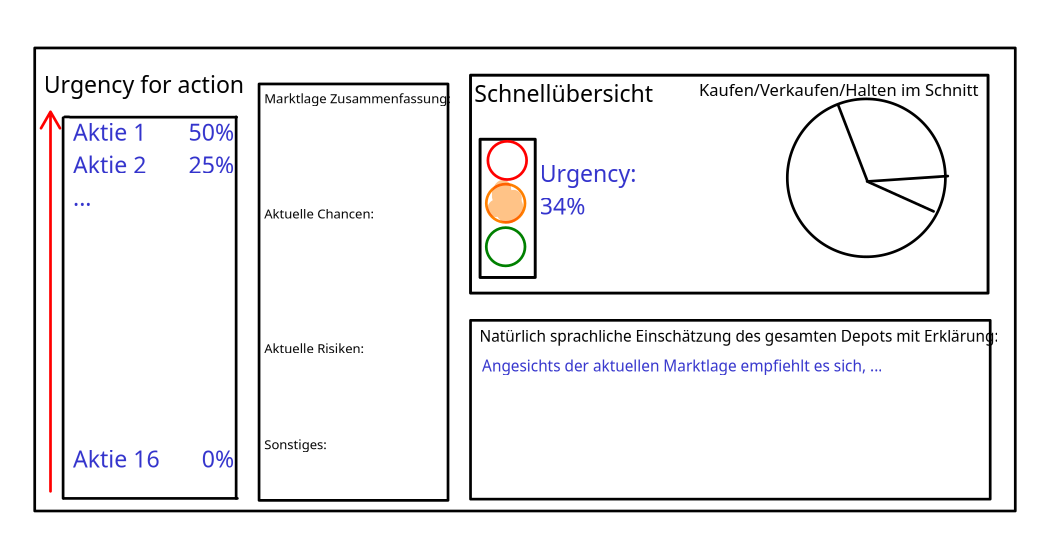
\includegraphics[width=0.85\textwidth]{assets/pictures/draft_portfolio_overview_frontend.png}
          \caption{Früher UI-Entwurf für die Portfolio-Übersicht zur Visualisierung}
          \label{fig:frontend_draft}
      \end{figure}

      Der Entwurf enthält Elemente wie eine \enquote{Urgency for Action}-Skala zur Priorisierung von Aktien, textuelle Risikobewertungen sowie natürlichsprachliche Zusammenfassungen.
      Besonders hervorzuheben ist die explizite Visualisierung der Unsicherheit und Bewertungsempfehlung (Kaufen/Verkaufen/Halten) in Form von Farben und Kreisdiagrammen.

      Diese Darstellungsweise basiert auf etablierten Gestaltungsprinzipien aus der HCI-Forschung, wonach kognitive Last minimiert werden kann, wenn Informationen multimodal, d.h. sowohl visuell als auch sprachlich, vermittelt werden. %To-Do: Quelle hinzufügen

      Neben dem Entwurf der Übersichtssicht gibt es noch die Sicht für das einzelne Wertpapier (siehe Abbildung~\ref{fig:frontend_draft_aktie}).

      \begin{figure}[H]
          \centering
          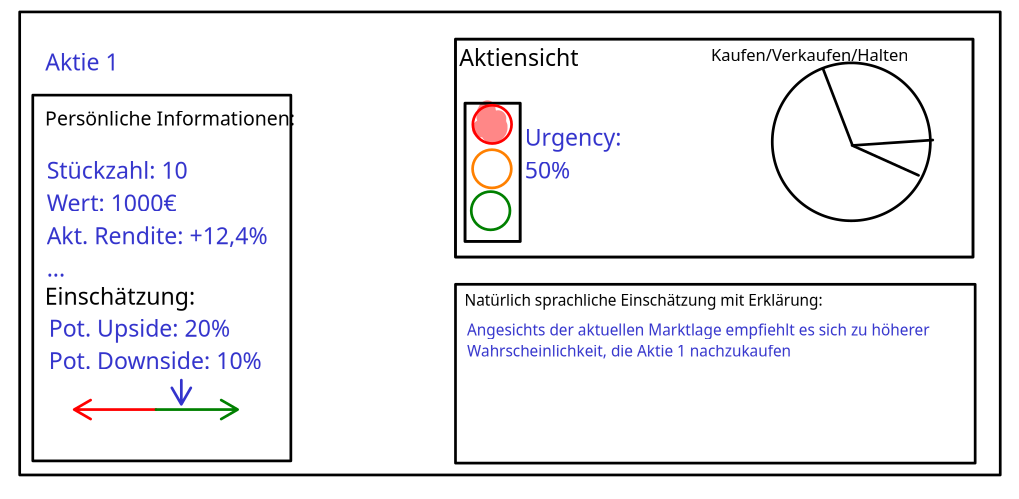
\includegraphics[width=0.85\textwidth]{assets/pictures/draft_portfolio_aktie_frontend.png}
          \caption{Früher UI-Entwurf für die Einzelwertpapiersicht zur Visualisierung}
          \label{fig:frontend_draft_aktie}
      \end{figure}

    \subsection{Implementierung und aktuelle Ausgestaltung}

      Auf Basis des oben dargestellten Drafts erfolgte eine iterative Umsetzung in HTML, CSS und JavaScript (vgl. Abschnitt~\ref{sec:entwicklung}).
      Die fertige Anwendung (siehe Abbildung~\ref{fig:frontend_live}) übernimmt viele der Grundideen des Entwurfs, wurde jedoch hinsichtlich Usability und technischer Umsetzbarkeit weiter verfeinert.
      Die Tabs erlauben eine navigation durch verschiedene Aktienansichten.

      \begin{figure}[H]
          \centering
          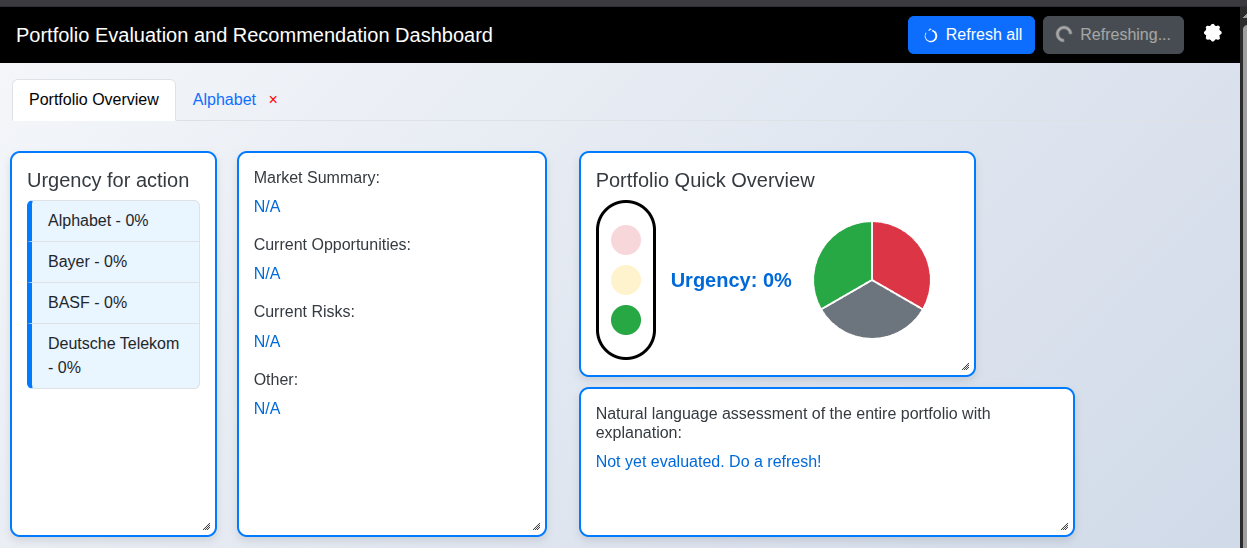
\includegraphics[width=0.9\textwidth]{assets/pictures/screenshot_frontend_vor_evaluierung.png}
          \caption{Live-System: Interaktive Web-Oberfläche zur Portfolioanalyse und Handlungsunterstützung}
          \label{fig:frontend_live}
      \end{figure}

      Die Anwendung zeigt aggregierte Portfolioinformationen und erlaubt auf Einzelwertebene eine genaue Analyse mit erklärender Textausgabe, die durch das LLM generiert wird.
      Dies ist besonders im Kontext der \textit{Erklärbarkeit} (\textit{Explainability}) entscheidend.
      Studien (To-Do: Studien benennen) zeigen, dass Nutzer algorithmischer Systeme nur dann fundierte Entscheidungen treffen oder Empfehlungen hinterfragen können, wenn die zugrundeliegenden Argumentationen transparent und zugänglich aufbereitet sind. %To-Do: Quelle hinzufügen

    \subsection{Wissenschaftliche Relevanz der UI im Kontext von Entscheidungsassistenz}

      Die Transparenz in Assistenzsystemen beschränkt sich nicht nur auf die algorithmische Modellierung, sondern betrifft maßgeblich auch die Präsentationsebene.
      Laut \cite{gunning2017explainable} ist eine erklärbare Benutzeroberfläche ein zentraler Bestandteil von XAI-Systemen (Explainable Artificial Intelligence), da sie den Brückenschlag zwischen Modelloutput und menschlichem Entscheidungsverhalten ermöglicht.
      Der Mehrwert einer fundierten UI liegt also nicht nur in der Ästhetik oder Bedienbarkeit, sondern in ihrer Fähigkeit, Vertrauen, Kontrolle und Nachvollziehbarkeit zu fördern.

      Zudem zeigen empirische Studien zur Mensch-Maschine-Interaktion (z.B. \cite{hoffman2018metrics}), dass die Qualität der Visualisierung einen direkten Einfluss auf das Nutzervertrauen und die Akzeptanz von KI-basierten Empfehlungen hat.
      Eine schlechte oder intransparente Visualisierung kann zu \textit{automation bias} oder kompletter Ablehnung der Empfehlung führen.


  \section{Zusammenfassung}

  Die Systemarchitektur des entwickelten Assistenzsystems ist bewusst modular und erweiterbar gestaltet.
  Der iterative Entwicklungsprozess ermöglichte eine schrittweise Einführung komplexerer Komponenten, ohne dabei die Wartbarkeit zu verlieren.
  Zukünftige Erweiterungen, wie die Integration fortgeschrittener Modelllogiken mit \texttt{LangChain} oder die Ablösung des Frontends durch reaktive Frameworks, können auf Basis dieser Architektur leicht implementiert werden.


\begin{comment}
\textbf{To-Dos:}
\begin{itemize}
  \item Modulare Darstellung der Systemkomponenten mit Schnittstellen
  \item Reproduzierbare Code-Beispiele für Kernfunktionen
  \item Diskussion technischer Limitationen (z. B. Latenzzeiten)
  \item Dokumentation der genutzten Frameworks/Tools (z. B. Ollama, Flask)

  \item\textbf{Ideen:}
  \begin{itemize}
    \item \textbf{Privacy-by-Design:} On-Device-Ansatz skizzieren
    \item \textbf{Plug-in-System:} Modularer Aufbau für Drittanbieter-Erweiterungen (z. B. mit FOSS Lösung Portfolio-Performance)
  \end{itemize}

\end{itemize}
\end{comment}